% \documentclass[CEJM,DVI]{cej} % use DVI command to enable LaTeX driver
\documentclass[CEJM,PDF]{cej} % use PDF command to enable PDFLaTeX driver
\usepackage{layout}
\usepackage{booktabs}
\usepackage{latexsym}
\renewcommand*\rmdefault{ppl}
\graphicspath{ {images/} }


\title{Predicting The Best Starting Price for Ebay Auctions}

\articletype{Course Project Milestone 2: Prediction on Item sale} % Research Article, Review Article, Communication, Erratum




\author{Jiacheng~Liao\inst{1},
        Yi~Wan\inst{1},
        Shuang~Zhou\inst{1},
        Zhaoyin~Zhu\inst{2}
       }

%\shortauthor{F. Author, S. Author}

\institute{\inst{1}
           Department of Computer Science, New York University, New York, NY 10012, USA
           \inst{2}
           Division of Biostatistics, NYU School of Medicine, New York, NY 10016, USA
          }

\abstract{Online auctions are one of the most popular methods to buy and sell items on the internet. With more than 100 million active users globally, eBay is the world’s largest online marketplace, where anyone can buy and sell anything. In order to successfully selling products on ebay, a reasonable starting price does not only determine whether the product will be sold or not but also affects the profit you can make from the transaction. In this project, we use the historical auction data collected from eBay from April 2013 to the first week of May 2013 which contains information about 296,048 successful and unsuccessful auctions. Different statistical models and machine learning algorithms will be utilized to study online auction patterns and predict the starting price that maximizes profits. Furthermore, we will compare the performance of different methods and summarize the pros and cons in different situations.
}

\keywords{Ebay Auction \*\ Predictive Analytics \*\ Data Mining}

%\msc{XXXXX, YYYYY}

\begin{document}
\maketitle
%\baselinestretch{2}
\section{Introduction (Data and Business Understanding) }

EBay is the world’s largest marketplace for sports autographs, the vast majority of the site’s membership uses it to buy and/or sell items via auction format. The ability to provide a method to estimate auction sale prices is desirable to this community. Members of most communities related to collectibles have reported they most often try to predict how much an auction would sell for by performing a search for item and manually calculating the average sales price. In this project, our first objective is to determine whether an auction listing will result in a sale. In addtion, we aim to predict the final sales price as well as the best starting price using data mining techniques.


\section{Data Preparation}

Data Preparation is an crucial and time-consuming part of our data mining project. It involves selecting data to include, cleaning data to improve data quality, constructing new data that may be required, integrating multiple data sets, and formatting data. We first preprocessed the downloaded data sets using shell scripts. To gain more experience on feature selection, we have performed the selection procedure on all three tools used in the class, RapidMiner, Weka and R. With different algorithms and parameters, we get slightly different but generally consistent results. 

\subsection*{Data Preprocessing}
Before any data can be used for later feature reduction and selection, we preprocessed our data sets. Here the tool we use is shell scripts. Initially, the raw data consists of training sets and test sets. Since we intend to do cross-validation on the whole data set, we merge all the separate data sets as one complete sets. Then we carefully go through all the data attributes and deleted all that obviously contain meaningless or irrelevant information to our analysis, such as ebayID, sellerName, etc. In addition, some attributes with ambiguous meanings are also discarded. 


\subsection{Feature Selection Using Weka}
First, we perform feature selection in Weka. To enable Weka to better handle the data, the first step is establishing a nominal class label. Below is a snapshot of the method we use here to discretize the class field here, which is originally a numeric type with value 0 and 1.

{\centering
    \vspace{3 mm}
    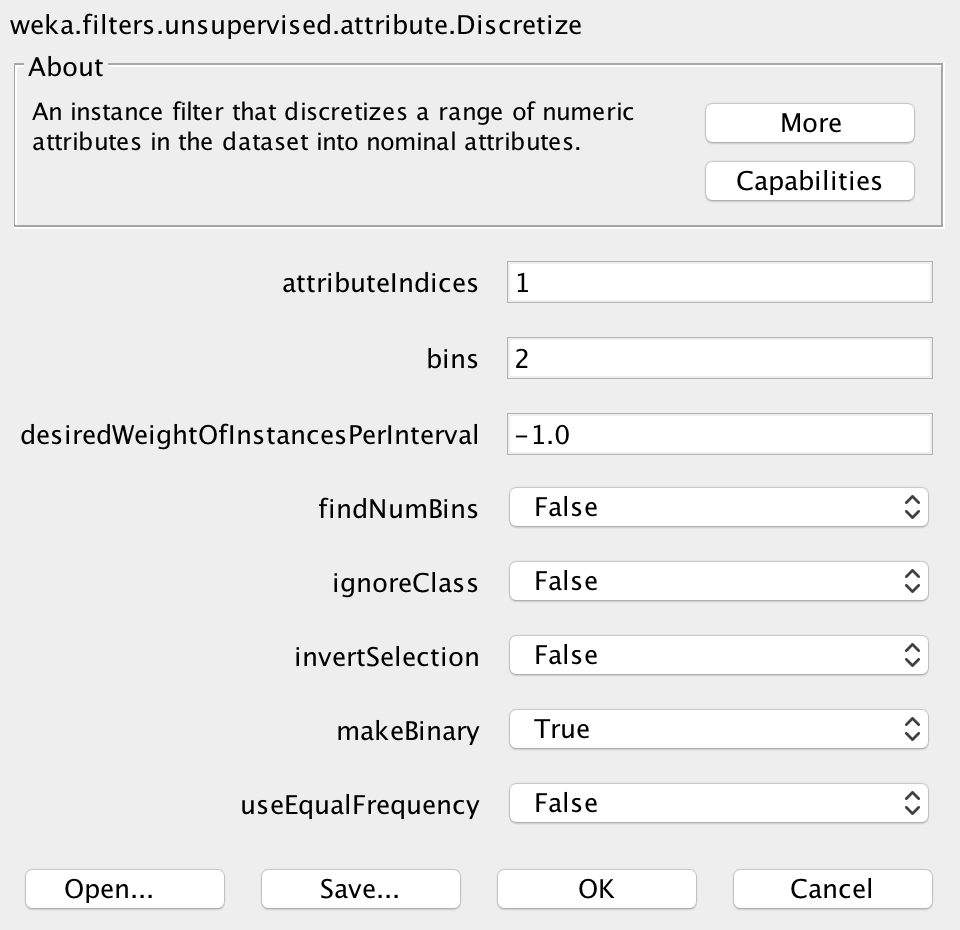
\includegraphics[scale=0.4]{weka-discretize_label_column.png}
    \par
}


Two algorithms are used in Weka: Information Gain and Feature Subset Selection. We first used Information Gain Algortihm and the result is as below. According to the information gain results we have, if we set the entropy threshold to 0.95, we will need the top 8 features.

{\centering
    \vspace{3 mm}
    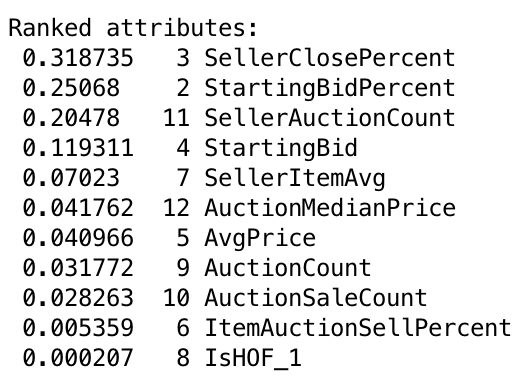
\includegraphics[scale=0.6]{weka-InfoGain.png}
    \par
}

Using the number of features obtained above, we set the number of features to 8 and try feature subset selection. We start with empty subset, and we use CfsSubsetEval as the evaluation of each subset, and we use GreedyStepWise search method, which basically select the best next feature based on current subset. Here is the result we get.

{\centering
    \vspace{3 mm}
    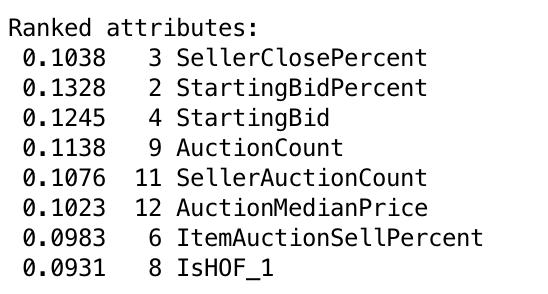
\includegraphics[scale=0.6]{weka-FilteredSubsetWithGreedyStepwise.png}
    \par
}


\subsection{Feature Selection Using R}
The caret R package provides tools automatically report on the relevance and importance of attributes in your data and even select the most important features for you. Here we perform three different feature selection method on our dataset, namely entropy based filter, Chi-square based filter and Correlation based filter. We apply all three filters to get a better sense of what attributes are more important, and we have the results below.\\
\begin{center}
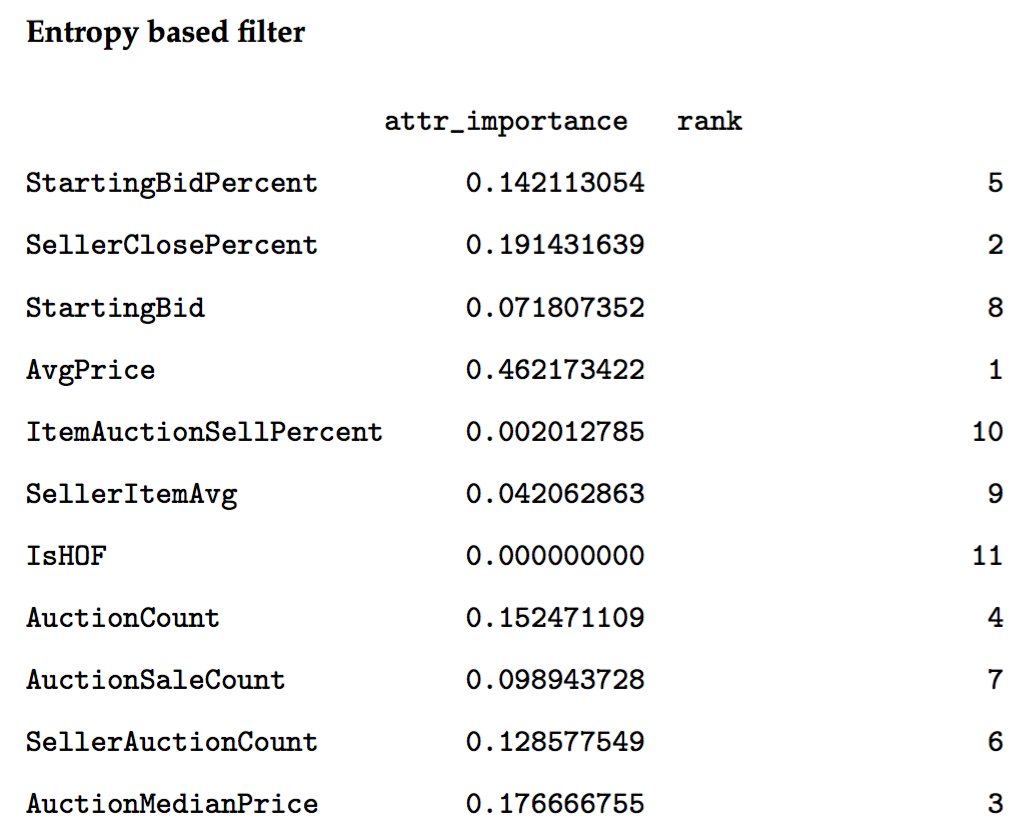
\includegraphics[scale=0.5]{entropy.png}\\
\mbox{}\\
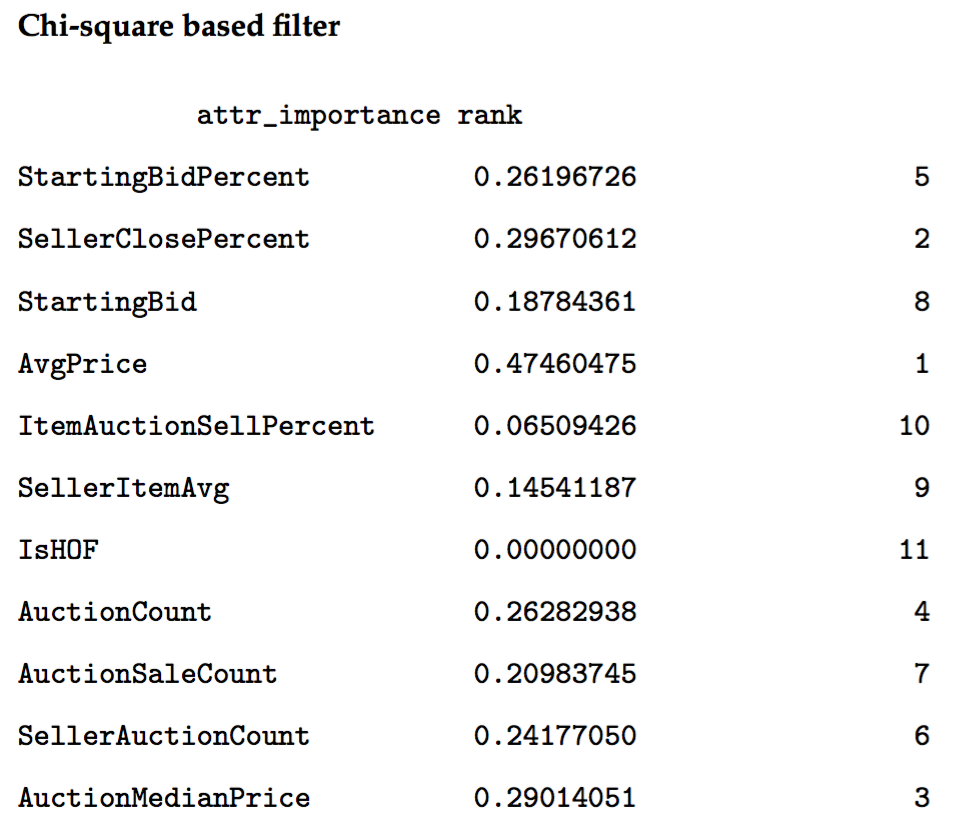
\includegraphics[scale=0.5]{chi-square.png}\hspace*{2em}
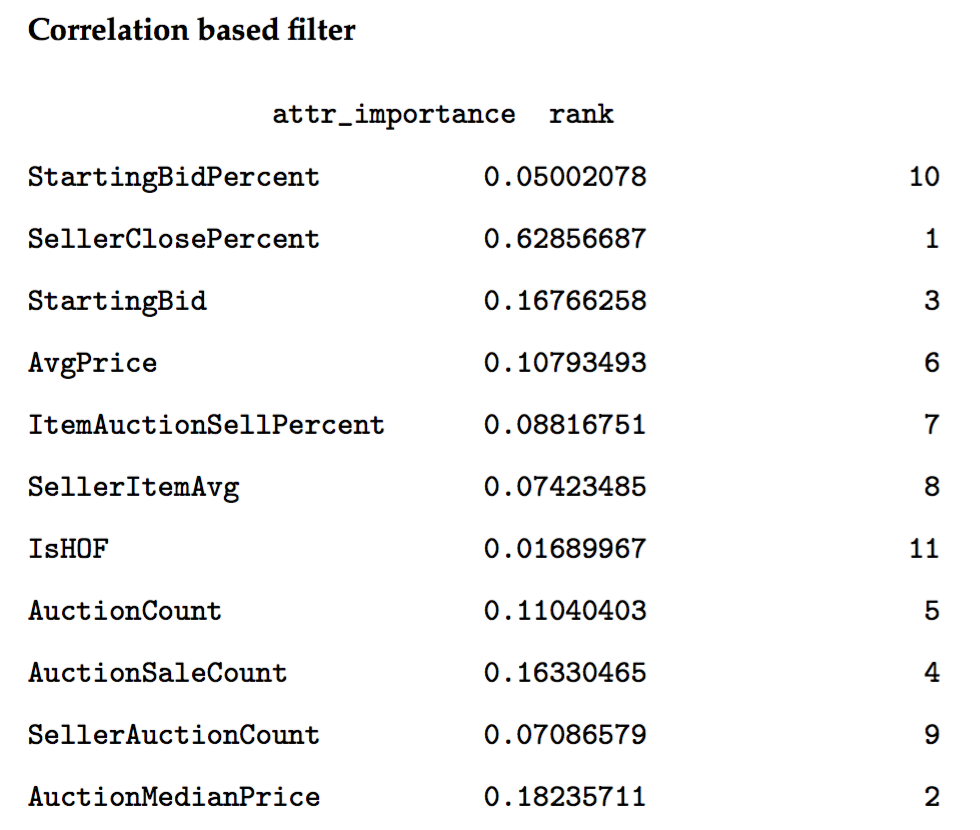
\includegraphics[scale=0.5]{correlation.png}\\
\end{center}
As a result, we summarize all the three different methods and compute average rank for each attribute. The result is presented in table \ref{r-rank}.


\begin{table}[h]
\centering
\caption{Feature Selection Using R Result}
\label{r-rank}
\begin{tabular}{@{}ccccc@{}}
\toprule
Attribute Name         & Entropy based filter & Chi-square based filter & Correlation based filter & Average Rank \\ \midrule
SellerClosePercent     & 2                    & 2                       & 1                        & 1.7     \\
AvgPrice               & 1                    & 1                       & 6                        & 2.7     \\
AuctionMedianPrice     & 3                    & 3                       & 2                        & 2.7     \\
AuctionCount           & 4                    & 4                       & 5                        & 4.3     \\
AuctionSaleCount       & 7                    & 7                       & 4                        & 6.0     \\
StartingBid            & 8                    & 8                       & 3                        & 6.3     \\
StartingBidPercent     & 5                    & 5                       & 10                       & 6.7     \\
SellerAuctionCount     & 6                    & 6                       & 9                        & 7.0     \\
SellerItemAvg          & 9                    & 9                       & 8                        & 8.7     \\
ItemAuctionSellPercent & 10                   & 10                      & 7                        & 9.0     \\
IsHOF                  & 11                   & 11                      & 11                       & 11.0    \\ \bottomrule
\end{tabular}
\end{table}

\subsection{Feature Selection Using RapidMiner}
First we choose a feature selection method from RapidMiner. Here we use Forward Selection. Forward selection operator selects the most relevant attributes of the given ExampleSet through a highly efficient implementation of the forward selection scheme. 

Forward selections uses wrapper method to select attributes. Basically, it starts with an empty attribute set. It them add one attribute to run the model and measures the performance. The process keep adding attributes to the model to see if there is performance gain. Depending on the parameter set, it will terminate until there is no performance improvement or no significant performance improvement. Here we also use cross-validation to measure the performance of the model as well as the current attributes set the operator.

For predicting the whether the given item can be sold or not, we use several classification algorithms, including: Naive Bayes, Decision Tree, Random Forest, Rule Induction, Neural net, Logistic Regression, Support Vector Machine. We will consider efficiency and prediction accuracy for each model to decide which one to adopt.

\subsubsection{Naive Bayes modeling}
{\centering
    A. The attribute weight
    \vspace{3 mm}
    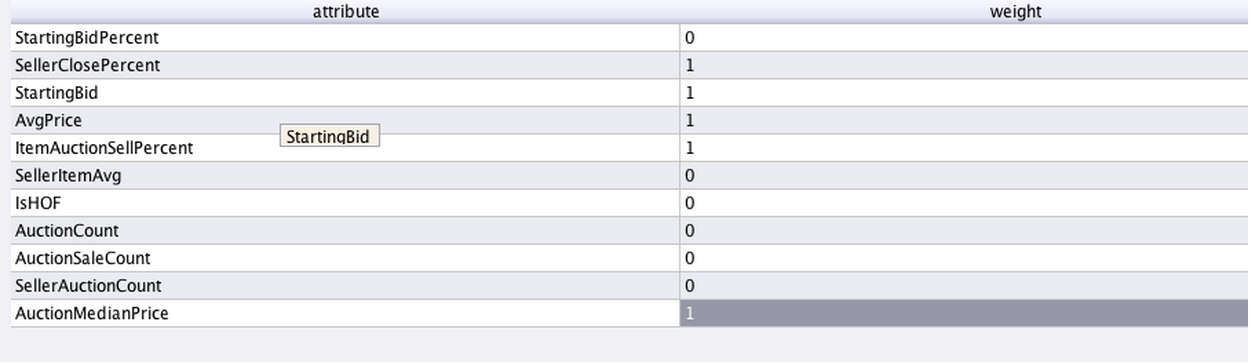
\includegraphics[scale=0.6]{rm-nb-aw.png}
    \par
}


{\centering
    B. The prediction model result and auc curve
    \vspace{3 mm}
    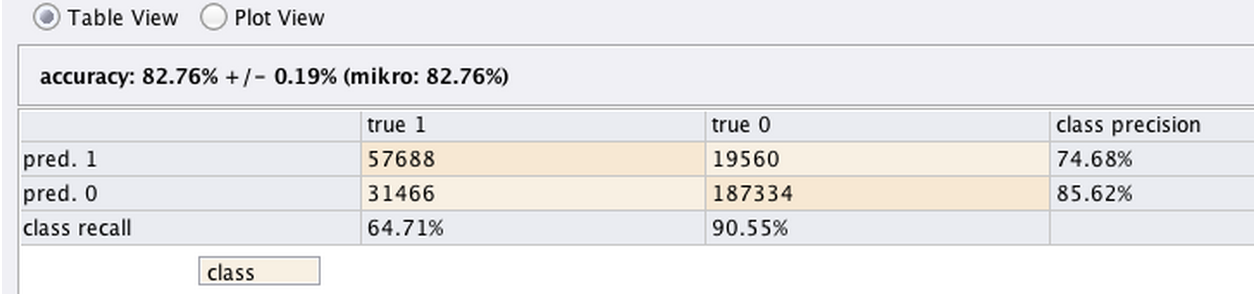
\includegraphics[scale=0.6]{rm-nb-perf.png}
    \vspace{3 mm}
    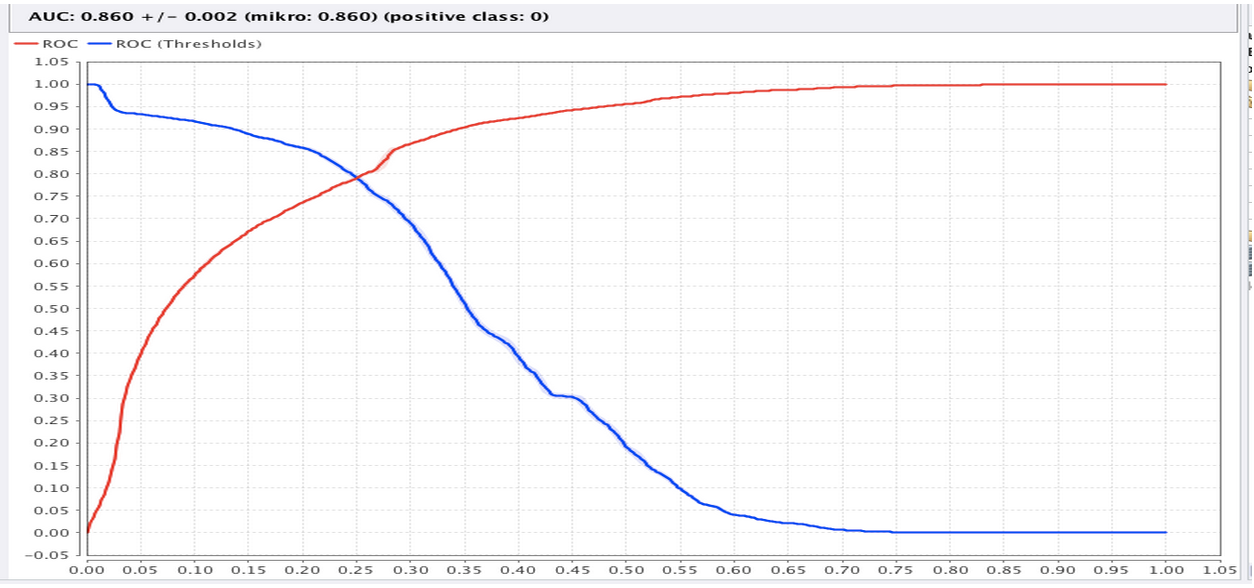
\includegraphics[scale=0.6]{rm-nb-auc.png}
    \par
}

\subsubsection{Decision Tree modeling}
{\centering
    A. The attribute weight
    \vspace{3 mm}
    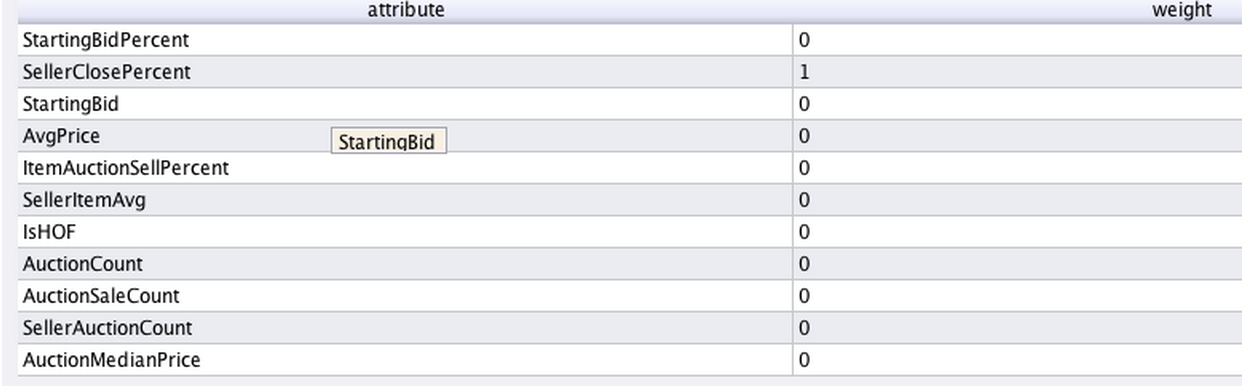
\includegraphics[scale=0.6]{rm-dec-aw.png}
    \par
}


{\centering
    B. The prediction model result and auc curve
    \vspace{3 mm}
    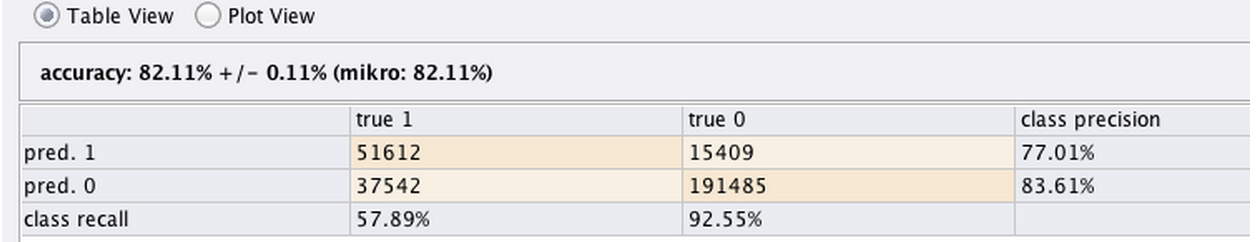
\includegraphics[scale=0.6]{rm-dec-perf.png}
    \vspace{3 mm}
    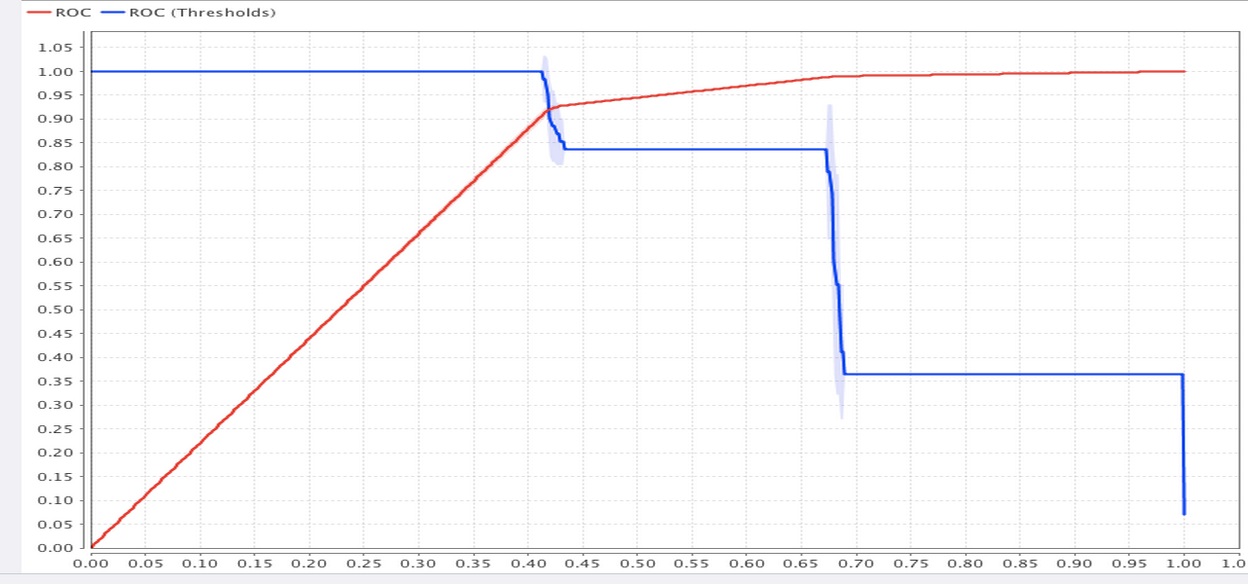
\includegraphics[scale=0.6]{rm-dec-auc.png}
    \par
}

\subsection{Other Trials}
The other methods including Random Forest, Rule Induction, Neural net, Logistic Regression, Support Vector Machine takes a very long time to finish (more than one hour). Since the dataset we are using is not very large, we consider them not suitable for our problem.


\subsection{Final Feature Selection}
To fairly select the features based on all three tools, we define an algorithm to integrate the results. An attributing score is assigned to each feature for final ranking, and the rules for assigning the score is as follow:\\
\begin{enumerate}
  \item In ranked result, the feature ranked $i$th is assigned a score of $12-i$, e.g. the highest feature gets a score of 11.
  \item In not ranked result, the features selected as useful is assigned a score of $8$ and others are assigned score of $0$.
  \item The final score is a summation of the results from all tools with all algorithms.
\end{enumerate}
The result computed is presented in table \ref{f-rank}.
 
\begin{table}[h]
\centering
\caption{Overall Feature Attributing Scores}
\label{f-rank}
\begin{tabular}{@{}lllll@{}}
\toprule
Attribute Name  & Weka Attributing Score & R Attributing Score & RapidMiner Attributing Score & \textbf{Overall Attributing Score} \\ \midrule
SellerClosePercent & 18   & 22  & 16 & 56   \\
AuctionMedianPrice & 12    & 20   & 8  & 40 \\
StartingBid  & 18    & 12  & 8  & 38 \\
AvgPrice  & 7  & 20  & 8  &  35   \\
StartingBidPercent  & 21  & 10  & 0 &  31  \\
AuctionCount & 13    & 16   & 0  & 29  \\
SellerAuctionCount & 17  & 8    & 0  & 25 \\
AuctionSaleCount  & 6     & 14  & 0  & 20  \\
ItemAuctionSellPercent & 7   & 4  & 8 & 19   \\
SellerItemAvg  & 8    & 6  & 0   & 14 \\
IsHOF  & 5    & 2  & 0  & 7  \\ \bottomrule
\end{tabular}
\end{table}

As indicated by Weka, the number of features we need to achieve a 0.95 information gain is 8, we narrowed the features down to the first 8 features in the table. And from here on, unless specified otherwise, we are using the reduced dataset with only these features.


\section{Modeling}

Modeling involves selecting suitable modeling techniques, generating test designs to validate the model, building predictive models and assessing these models.\\
\\
A predictive model is a mathematical function that predicts the value of some output variables based on the mapping between input variables. Historical data is used to train the model to arrive at the most suitable modeling technique. For example, a predictive model might predict the risk of developing a certain disease based on patient details. Some commonly used modeling techniques are as follows: Regression analysis that analyzes the relationship between the response or dependent variable and a set of independent or predictor variables. Decision trees that help explore possible outcomes for various options. Cluster analysis that groups objects into clusters to look for patterns. Association techniques that discover relationships between variables in large databases.\\
\\
Modeling in this project consists of two parts. In the first part, we try to build a model to predict whether an item can be sold or not. And in the second model, we try to predict a best starting price that maximize the final sale price.\\

\subsection{Modeling for Sale / No Sale}
In all three tools here, we tried to use different type of classification algorithms to decide whether items can be sold or not based on some information of item across Ebay.
\\
\subsubsection{Modeling in Weka}
To compare the effectiveness of different algorithms, we decided to use F measure as the criteria to measure performances of each model. The label of interest is sold (denoted by 1) and not sold (denoted by 0). NB classifier is the first algorithm we try. Naive Bayes classifiers are a family of simple probabilistic classifiers based on applying Bayes' theorem with strong (naive) independence assumptions between the features. It's as straightforward as it gets. \\
\\
Another algorithm we use is Logistic Regression, Logistic regression measures the relationship between the categorical dependent variable and one or more independent variables by estimating probabilities using a logistic function, which is the cumulative logistic distribution. It fits very well in our situation, and it's a fast model to train and use. Both NB classifier and Logistic Regression are applied over the dataset in Weka, and results are presented in table \ref{weka-model}.\\

\begin{table}[h]
\centering
\caption{Model Comparison in Weka}
\label{weka-model}
\begin{tabular}{@{}|l|l|@{}}
\toprule
\hline
Model Name  & F measure \\ \midrule
\hline
Naive Bayes & 0.639   \\
\hline
Logistic Regression  & 0.837 \\ \bottomrule
\hline
\end{tabular}
\end{table}

Obviously Logistic Regression model works much better than NB model for this dataset, with a F measure of 0.837. But we will continue to examine different models with other tools.\\

\subsubsection{Modeling in RapidMiner}
In RapidMiner, models we tried include Naive Bayes, Random Forest, Decision Tree, Logistic Regression, Neural Network. Some of the models can't finish in reasonable time due to the RapidMiner design that enforce us to add ``Performance" module into the process, which noticeably increases the running time. So as a result, we only present Naive Bayes, Random Forest, and Decision Tree models here. \\
\\
A decision tree is a decision support tool that uses a tree-like graph or model of decisions and their possible consequences, including chance event outcomes, resource costs, and utility. The decision tree algorithm comes with a ``depth" parameter and a evaluation algorithm. For the evaluation algorithm, we used Gain Ratio.\\
\\
Random forests are an ensemble learning method for classification, regression and other tasks, that operate by constructing a multitude of decision trees at training time and outputting the class that is the mode of the classes (classification) or mean prediction (regression) of the individual trees. Random forests correct for decision trees' habit of overfitting to their training set. See table \ref{rm-model} for all results.\\ 

\begin{table}[h]
\centering
\caption{Model Comparison in Weka}
\label{rm-model}
\begin{tabular}{@{}|l|l|@{}}
\toprule
\hline
Model Name  & F measure \\ \midrule
\hline
Naive Bayes & 0.629   \\
\hline
Decision Tree (Depth = 5) & 0.8223\\
\hline
Decision Tree (Depth = 10) & 0.8334 \\
\hline
Decision Tree (Depth = 50) & 0.8334 \\
\hline
Random Forest & 0.7912 \\ \bottomrule
\hline
\end{tabular}
\end{table}

In Decision Tree classifier, to obtain the best result, we tried multiple depths from 5 to 50, the accuracy grows a little with the depth at first, and then stays the same when the depth is greater than 10. Intuitively this makes sense because as the depth go up, it's more likely to find relations between each attribute and the label, but given there're only 8 features in total, the depth wouldn't matter too much after it exceeds the number of features.\\
\\
In Random Forest algorithm, a somewhat surprising discovery is that the overall accuracy is slightly lower than Decision Tree algorithm, because given that Random Forest classifier is a much more complicated algorithm, we suppose it should do better. But as a property of Random Forest, it tends to get rid of overfitting behaviors of decision trees, and the accuracy here is computed based on the exact same dataset we used for training the classifier. Therefore, this is an acceptable loss. And we will find out which one is more accurate when we apply them on unknown datasets.\\

\subsubsection{Modeling in R}
Just to gain experience on as many tools as possible, we also try to build our model with R. We chose two algorithms to experiment with, namely, Logistic Regression (just to compare results with RapidMiner and Weka) and K-Nearest Neighbors. The k-Nearest Neighbors algorithm (or K-NN for short) is a non-parametric method used for classification and regression. In most cases, the input consists of the $k$ closest training examples in the feature space. The output is a class membership. An object is classified by a majority vote of its neighbors, with the object being assigned to the class most common among its $k$ nearest neighbors ($k$ is a positive integer, typically small). If $k$ = 1, then the object is simply assigned to the class of that single nearest neighbor. We are able to find Logistic Regression algorithm from the famous ``Generalized Linear Model" package in R, and we also find a very authoritative implementation of KNN algorithm in \_\_\_\_\_\_\_\_. Logistic Regression Result from R is in table \ref{r-lr}:\\

\begin{table}[h]
\centering
\caption{Coefficient Table for Logistic Regression}
\label{r-lr}
\begin{tabular}{@{}|l|r|@{}}
\toprule
\hline
Entry Name  & Coefficient \\ \midrule
\hline
Intercept & -1.760e+00   \\
\hline
StartingBidPercent & -8.886e-01 \\
\hline
SellerClosePercent & 4.829e+00  \\
\hline
StartingBid & -9.735e-03  \\
\hline
AvgPrice & -9.735e-05 \\
\hline
AuctionCount & -1.670e-03   \\
\hline
AuctionSaleCount & 5.457e-03  \\
\hline
SellerAuctionCount & 1.328e-05   \\
\hline
AuctionMedianPrice & 9.477e-03  \\ \bottomrule
\hline
\end{tabular}
\end{table}

To interpret the table, let's say $e_1, e_2, ..., e_n$ are $n$ entries (features), and $c_0, c_1, c_2, ..., c_n$ are $n$ corresponding coefficients with $c_0$ being the intercept, or constant, in this formula, computed by the algorithm. Then, for a given instance $x$, the label of this instance can be generated with:
$$L(x) = c_0 + \sum_{i=1}^{n}e_i\times c_i$$
We can't obtain much information by simply looking at the expression, although some may wonder the importance of each feature is indicated by the absolute value of each coefficient. That's not true in most cases, as all features have different magnitudes and coefficients play the role as mitigator among all those features. We evaluate the model, and the F measure reaches 0.89.\\
\\
For K-NN, we try to run it with different number of neighbors in order to find the ``magic number", and results are presented in table \ref{r-knn}.

\begin{table}[h]
\centering
\caption{K-NN With Different Number Of Neighbors}
\label{r-knn}
\begin{tabular}{@{}|l|l|@{}}
\toprule
\hline
Number of Neighbors  & F measure \\ \midrule
\hline
5 & 0.829   \\
\hline
7  & 0.830  \\
\hline
9  & 0.830  \\ \bottomrule
\hline
\end{tabular}
\end{table}

It appears that number of neighbors doesn't seem to make much of a difference here, but the overall accuracy is very solid.\\

\subsubsection{Final Model Selection}
Considering all models we've tried, we decide to go with Logistic Regression model. It performs the most stably and can achieve a near 90 percent accuracy according to our cross-validation result from R.

\subsection{Modeling For Best Starting Price}
To be finished


\section{Team Members Responsibilities and Plan for the Next Phase}

Right now, all group members are actively participate in the project. An approximate list of each team members' responsibility is:
\begin{itemize}
\item Jiacheng Liao: data preprocessing, report write-up
\item Yi Wan: data preprocessing, feature selection in RapidMiner
\item Shuang Zhou: data preprocessing, feature selection in Weka
\item Zhaoyin Zhu: data preprocessing, feature selection in R
\end{itemize}

For the next phase,we intend to build different models to make predictions. We plan to apply various statistical machine learning model and use cross-validation to test each model. Also, we would study some economic aspects of the auction theory to help us build the model.


\section{Evaluation (ToDo)}
Evaluation involves evaluating the results against the business success criteria defined at the beginning of the project.


\section{Deployment (ToDo)}
Deployment involves consolidating the findings, determining what might be deployed and planning the monitoring and maintenance required to keep the model relevant.

\section{Conclusion (ToDo)}
TODO


\section*{Acknowledgements}

The author(s) would like to thank some institutions for support and so on.


\begin{thebibliography}{9}

\bibitem{data-mining}Han, Jiawei, Micheline Kamber, and Jian Pei.\textit{ Data mining: concepts and techniques: concepts and techniques}. Elsevier, 2011.

\bibitem{mining-mass} Rajaraman, Anand, and Jeffrey D. Ullman. \textit{Mining of massive datasets}. Vol. 77. Cambridge: Cambridge University Press, 2012.

\bibitem{pre-dummy} Bari, Anasse, Mohamed Chaouchi, and Tommy Jung. \textit{Predictive analytics for dummies}. John Wiley \& Sons, 2014.	

\bibitem{lecture} Bari, Anasse. Predictive Analytics Course Lecture Notes. 2015 Fall.

\bibitem{r-feature}  Brownlee, Jason. Feature Selection with the Caret R Package. http://machinelearningmastery.com/feature-selection-with-the-caret-r-package/

\bibitem{ebay-auction} Grossman, Jay. Predicting eBay Auction Sales with Machine Learning.

Retrived from http://jaygrossman.com/post/2013/06/10/Predicting-eBay-Auction-Sales-with-Machine-Learning.aspx


\end{thebibliography}

\end{document}
